131. \begin{figure}[ht!]
\center{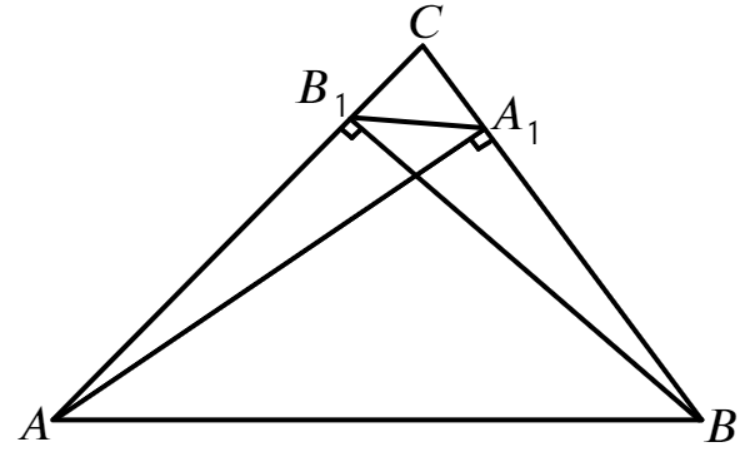
\includegraphics[scale=0.35]{g8-131.png}}
\end{figure}\\
В четырёхугольнике $AB_1A_1B$ угол, образованный стороной $AB_1$ и диагональю $BB_1,$ равен углу, образованному стороной $BA_1$ и диагональю $AA_1,$ значит он является вписанным. Тогда $\angle B_1A_1B+\angle BAC=180^\circ,\ \angle B_1A_1B=180^\circ-32^\circ=148^\circ.$ Угол $\angle CA_1B_1$ является смежным к нему, значит $\angle CA_1B_1=180^\circ-148^\circ=32^\circ.$\\
